\documentclass[12pt]{article}
\usepackage[pdftex]{graphicx}
\usepackage{url}
\usepackage{setspace}
\usepackage{makeidx}
\usepackage[utf8]{inputenc}
\usepackage{fancyhdr}
\usepackage{layout}
\usepackage{float}
\usepackage{graphicx}
\usepackage[a4paper,pdftex]{geometry}	% Use A4 paper margins
\usepackage[english,spanish]{babel}
\usepackage{xcolor} % Required for specifying custom colors
\usepackage{fix-cm} % Allows increasing the font size of specific fonts beyond LaTeX default specifications

\DeclareGraphicsExtensions{.pdf,.png,.jpg}

\setlength{\oddsidemargin}{0mm} % Adjust margins to center the colored title box
\setlength{\evensidemargin}{0mm} % Margins on even pages - only necessary if adding more content to this template

\setlength{\voffset}{-1.2cm}
\setlength{\textheight}{650pt}
\setlength{\parindent}{0pt}
\renewcommand{\baselinestretch}{1.5}
\definecolor{grey}{rgb}{0.9,0.9,0.9} % Color of the box surrounding the title - these values can be changed to give the box a different color	

\pagestyle{fancy}
\fancyhf{}
\lhead{A Fireball for Your Friends}
\rhead{Concept Proposal Document}
\rfoot{\thepage}

\makeindex

\begin{document}

\pagestyle{empty} % Remove page numbering on this page

%----------------------------------------------------------------------------------------
%	TITLE SECTION
%----------------------------------------------------------------------------------------

\colorbox{grey}{
	\parbox[t]{1.0\linewidth}{
		\fontsize{50pt}{30pt}\selectfont % The first argument for fontsize is the font size of the text and the second is the line spacing - you may need to play with these for your particular title
		\vspace*{0.7cm} % Space between the start of the title and the top of the grey box
		
		A Fireball \\ 
		for Your Friends \\ 
        \fontsize{30pt}{34pt}\selectfont
        Concept Proposal Document		
		\par
		
		\vspace*{0.4cm} % Space between the end of the title and the bottom of the grey box
	}
}

\vspace*{0.4cm} 
{\large Un \textbf{juego de duelos mágicos multijugador en 3ª persona}}

\begin{spacing}{0.6}
Target: \textit{chicos entre 16-22 años, amantes de los juegos competitivos, mid-core} 

Plataforma: \textit{Nintendo Switch (consola y portátil)}
\end{spacing}


\begin{figure}[h]
    \centering
    
\includegraphics[width=0.6\textwidth]{fireball}
\end{figure}

\vfill % Space between the title box and author information

{\centering \hfill \copyright 2016 Pedro Montoto García} \\

%----------------------------------------------------------------------------------------

\cleardoublepage

\setlength{\voffset}{0cm}
\setlength{\parindent}{1cm}

\section{Concepto General}
\pagestyle{fancy}
\setcounter{page}{1}

Un juego multijugador (pantalla partida y online) en tercera persona donde dos equipos cada uno con de 1 a 3 magos duelean en un pequeño escenario usando hechizos variados y espectaculares. Cada jugador deberá componer su biblioteca de hechizos en cada encuentro, escogiéndolos según la utilidad que tengan para contrarrestar al enemigo y sinergizar con sus aliados. 

Cada encuentro tendrá sus objetivos, i.e. aniquilación, capturar la bandera, defender un objetivo, football..., y su duración será corta, i.e. entre 5 y 10 minutos, para asegurar que todo el mundo pueda disfrutar de al menos una partida rápida, pero que ésta sea intensa.

La experiencia de juego se centra en hacer que el jugador sienta su maestría al derrotar a enemigos usando los diferentes hechizos, evitándolos a su vez. El loop de juego principal estará en dominar los diferentes hechizos y sus sinergias via el empoderamiento del jugador.

\begin{figure}[h]
    \centering
    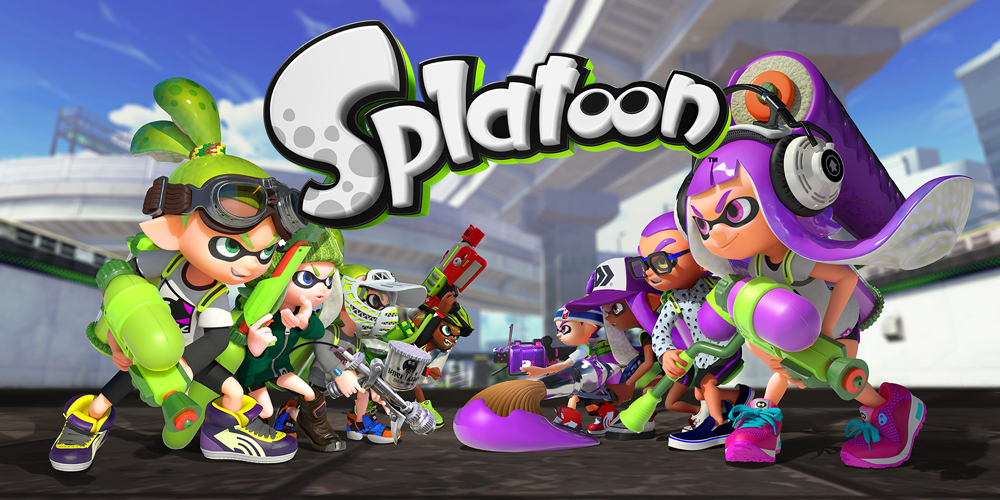
\includegraphics[width=\textwidth]{splatoon}
    \caption{Splatoon es una de las referencias principales del gameplay}
\end{figure}

\newpage

\section{Visual Appeal}

\subsection{Character appeal}

Dado que no planteamos un modo historia de un sólo jugador, sino que la historia se ve símplemente como un extra que añade una capa de profundidad al modo multijugador como flavor text de hechizos y personalizaciones, en este apartado nos centraremos en conseguir una estética agradable, personal y que envejezca bien (i.e. Team Fortress, Overwatch) dado que siendo multijugador nuestro planteamiento es alargar la vida del juego lo máximo posible. Para ello un estilo visual y narrativo de dibujos animados es un estándar de facto en la industria.

Otro punto importante en los gráficos es la variedad de elementos de personalización del personaje jugador, de los entornos y de los efectos de hechizo.

\subsection{Scope of Visual Effects: Visual Variety}

Estamos orientados a hacer este juego lo más espectacular y variado posible. Siendo la variedad de hechizos uno de nuestros Unique Selling Points haremos cada hechizo fácilmente reconocible por sus efectos visuales al mismo tiempo que las combinaciones que cada jugador escogerá en sus partidas sean únicas en cada una. Para conseguir ésto se utilizará todo el potencial de efectos especiales, efectos de partículas y post-procesado de pantalla completa.

\subsection{Environment Appeal}

Los entornos serán simples pero rápidamente identificables. La idea es que los entornos sirvan para aumentar la variedad de situaciones que el jugador afrontará durante sus partidas: aunque se ponga la atención en su atractivo visual éste no es el objetivo principal de nuestros entornos de juego.

\newpage  

\section{Innovation}        

\subsection{Technical Innovation}

El juego está planteado para la Nintendo Switch, que es una consola nueva que se lanzará en 2017. Dado que será uno de los primeros juegos de esta consola es probable que se descubra aparataje tecnológico fuera de las herramientas básicas (Nintendo Switch SDK) que Nintendo proveerá.

\subsection{Gameplay Innovation}

El género shooter en 3ª persona con elementos de fantasía no ha sido tradicionalmente usado en consolas de Nintendo, lo que ofrece una experiencia novedosa a los fans de esta compañía.

\subsection{Theme/Narrative/Concept Innovation}

La narrativa no es un elemento importante en este juego. Sin embargo el hecho de que se pueda contar una historia indirectamente mediante los elementos que el jugador mezclará durante su experiencia de juego (principalmente hechizos y skins) hace que sea una opción a explorar.

Como ya se ha indicado la combinación de género y gameplay presentada sí es novedosa.

\subsection{New IP}

A Fireball for Your Friends es una nueva IP sin relación alguna con otros productos existentes en el mercado.

\newpage

\section{Gameplay Features}     

\subsection{Reward systems}

\begin{itemize}
\item Un sistema de desbloqueo de habilidades irá guiando al jugador de hechizos más simples a otros más complejos, para que su curva de aprendizaje sea menos costosa. Sistemas similares se usan en Heroes of the Storm y LOL, o el modo ``héroes simples'' en DOTA.
\item Como extensión del sistema previo, un subsistema de niveles y puntos de experiencia por partida finalizada recompensará al jugador con sistemas de personalización variados. Se establecerán quests diarias con recompensas de experiencia extras para recompensar a los jugadores que asisten al juego más regularmente.
\item Un modo de juego competitivo proveerá a los jugadores más hardcore de un modo de juego más acorde a sus gustos.
\end{itemize}     

\subsection{Modes of play}

El juego ofrece un modo de práctica contra maniquíes de mago, para probar y practicar habilidades. El core del juego será la elección de ``modo de dificultad'' multijugador:

\begin{description}
\item[Quick Play:] Modo ``Casual'' de partidas rápidas
\item[Competitivo:] Modo ``Serio'' donde se asume mayor habilidad y coordinación dentro del equipo
\end{description}

\newpage

En Quick Play o Competitivo pueden jugarse los siguientes modos:

\begin{description}
\item[Exterminación:] Equipos de Magos intentan matarse unos a otros. Gana el equipo que tenga más miembros vivos con un límite de tiempo gana.
\item[Capturar la Bandera:] Existen bases para cada equipo y cada una guarda una bandera. El objetivo es entrar en la base enemiga y llevar la bandera enemiga a la base propia. Gana el equipo que más puntos tenga al final del límite de tiempo.
\item[Football:] El entorno de juego es un campo libre con dos ``porterías'' en los extremos, cada una de un equipo. El modo de juego consiste en combinar la lucha con el uso de los hechizos para meter la pelota en la portería contraria. Gana el equipo que más goles tenga al final del límite de tiempo.
\end{description}

\subsection{Audio ambition}

Sin pretensiones excesivas en la banda sonora, se pondrá un especial cuidado en que los efectos de sonido estén correctamente mezclados y generados para que ayuden a la identificación más rápida de la situación de la partida.

\subsection{HD Support}

Daremos soporte a monitores de alta resolución por defecto.

\subsection{Exclusive Content}

Más allá del propio contenido del juego no se prevén integraciones de contenido con Nintendo u otros juegos.

\newpage  

\section{Game Dynamics}

\subsection{Physics}

El juego incluye un sistema de físicas extendido para poder procesar todos los tipos de hechizo que se nos puedan ocurrir.

\subsection{AI}

Dado que la generación de IA es un proceso costoso en un juego tan variado como éste no se incluirá ningún tipo de IA avanzada para jugar contra el jugador. Se incluye un sistema de maniquíes de práctica simples para que el jugador pueda familiarizarse con sus hechizos de ataque y defensa.

\subsection{Environmental Interaction}

Para incrementar la inmersión del jugador y favorecer la creación y evolución de estrategias de juego se incluirán elementos destructibles en los niveles de juego (i.e. paredes, árboles etc.).

\subsection{Object Interaction}

No hay interacción con objetos de juego más allá de la configuración de habilidades y apariencia.

\subsection{Avatar Evolution}

La personalización del avatar y la adquisición de hechizos cada vez más complejos es la base del gameplay.     

\subsection{Camera Behavior}

Se provee una cámara en 3ª persona básica, con gestión de colisiones con objetos del entorno y controlada mediante el mando de Switch (ver sección Control).

\newpage      

\section{Control}

\subsection{Configuration}

\begin{figure}[h]
    \centering
    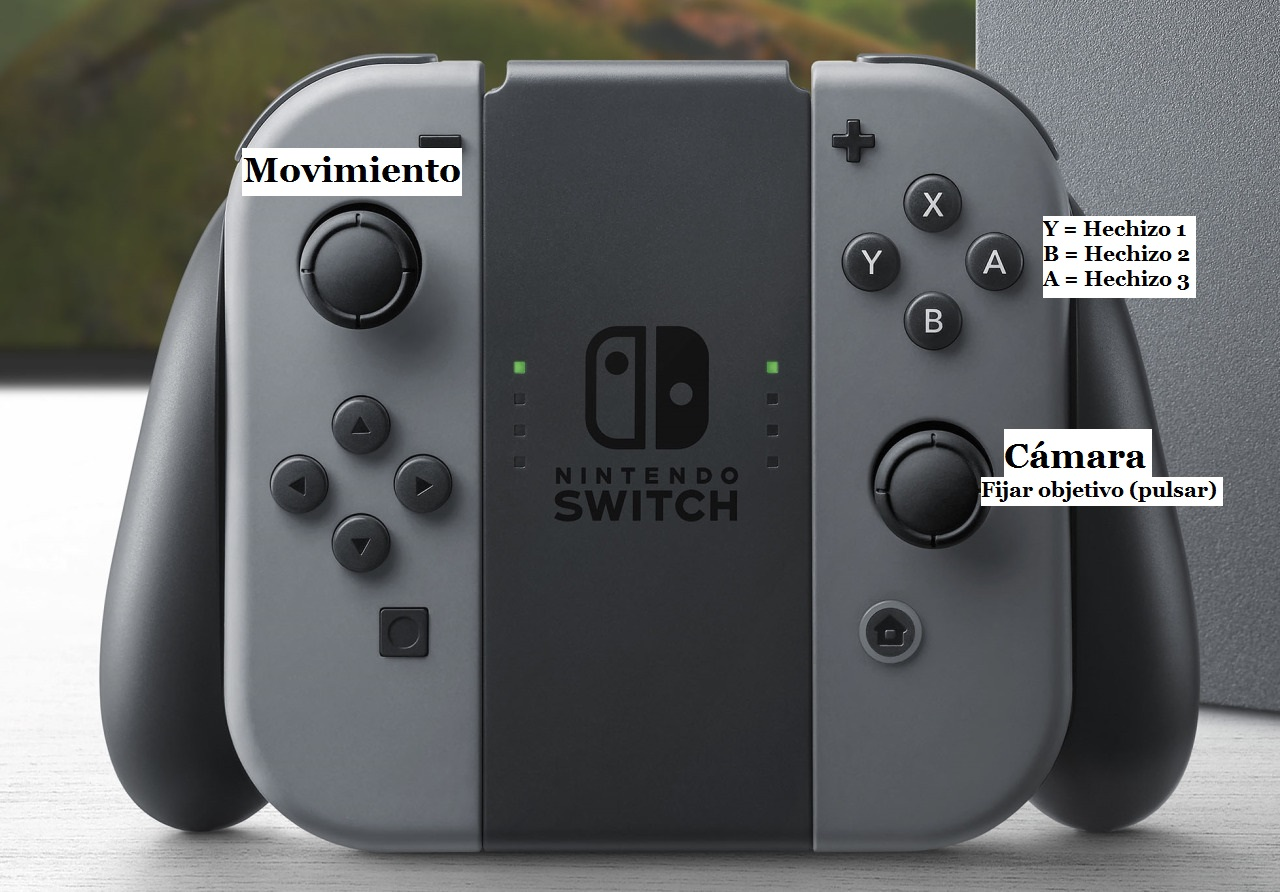
\includegraphics[width=\textwidth]{controller}
    \caption{El control será completamente configurable, con estos valores por defecto en juego}
\end{figure}

\subsection{Interface / HUD}

La HUD es completamente minimalista: sólo se enseña la salud restante, los hechizos elegidos y una crosshair para apuntar.        

\newpage

\section{Game Structure}              

\subsection{Tutorial and training}

Se diseña un nivel de tutorial (ver abajo) en el que el jugador aprenderá los hechizos básicos: la Bola de Fuego, el Escudo Reflector y Cura guiado por un narrador. Una vez el jugador haya superado o rechazado jugar este nivel de tutorial se le permitirá entrar en el modo online y adquirir nuevas habilidades que podrá probar dentro del mismo nivel de tutorial.

\subsection{Accessibility}

Un modo gráfico extra adapta la visibilidad de pantalla para personas con daltonismo.

\subsection{Level Design}

El diseño de los niveles es minimalista y simplificado, para dejar paso a gameplay emergente dadas las habilidades y movimientos de los participantes. Se presenta aquí el diseño básico de un nivel del modo tutorial y otro nivel del modo Capturar la Bandera.

\begin{figure}[H]
    \centering
    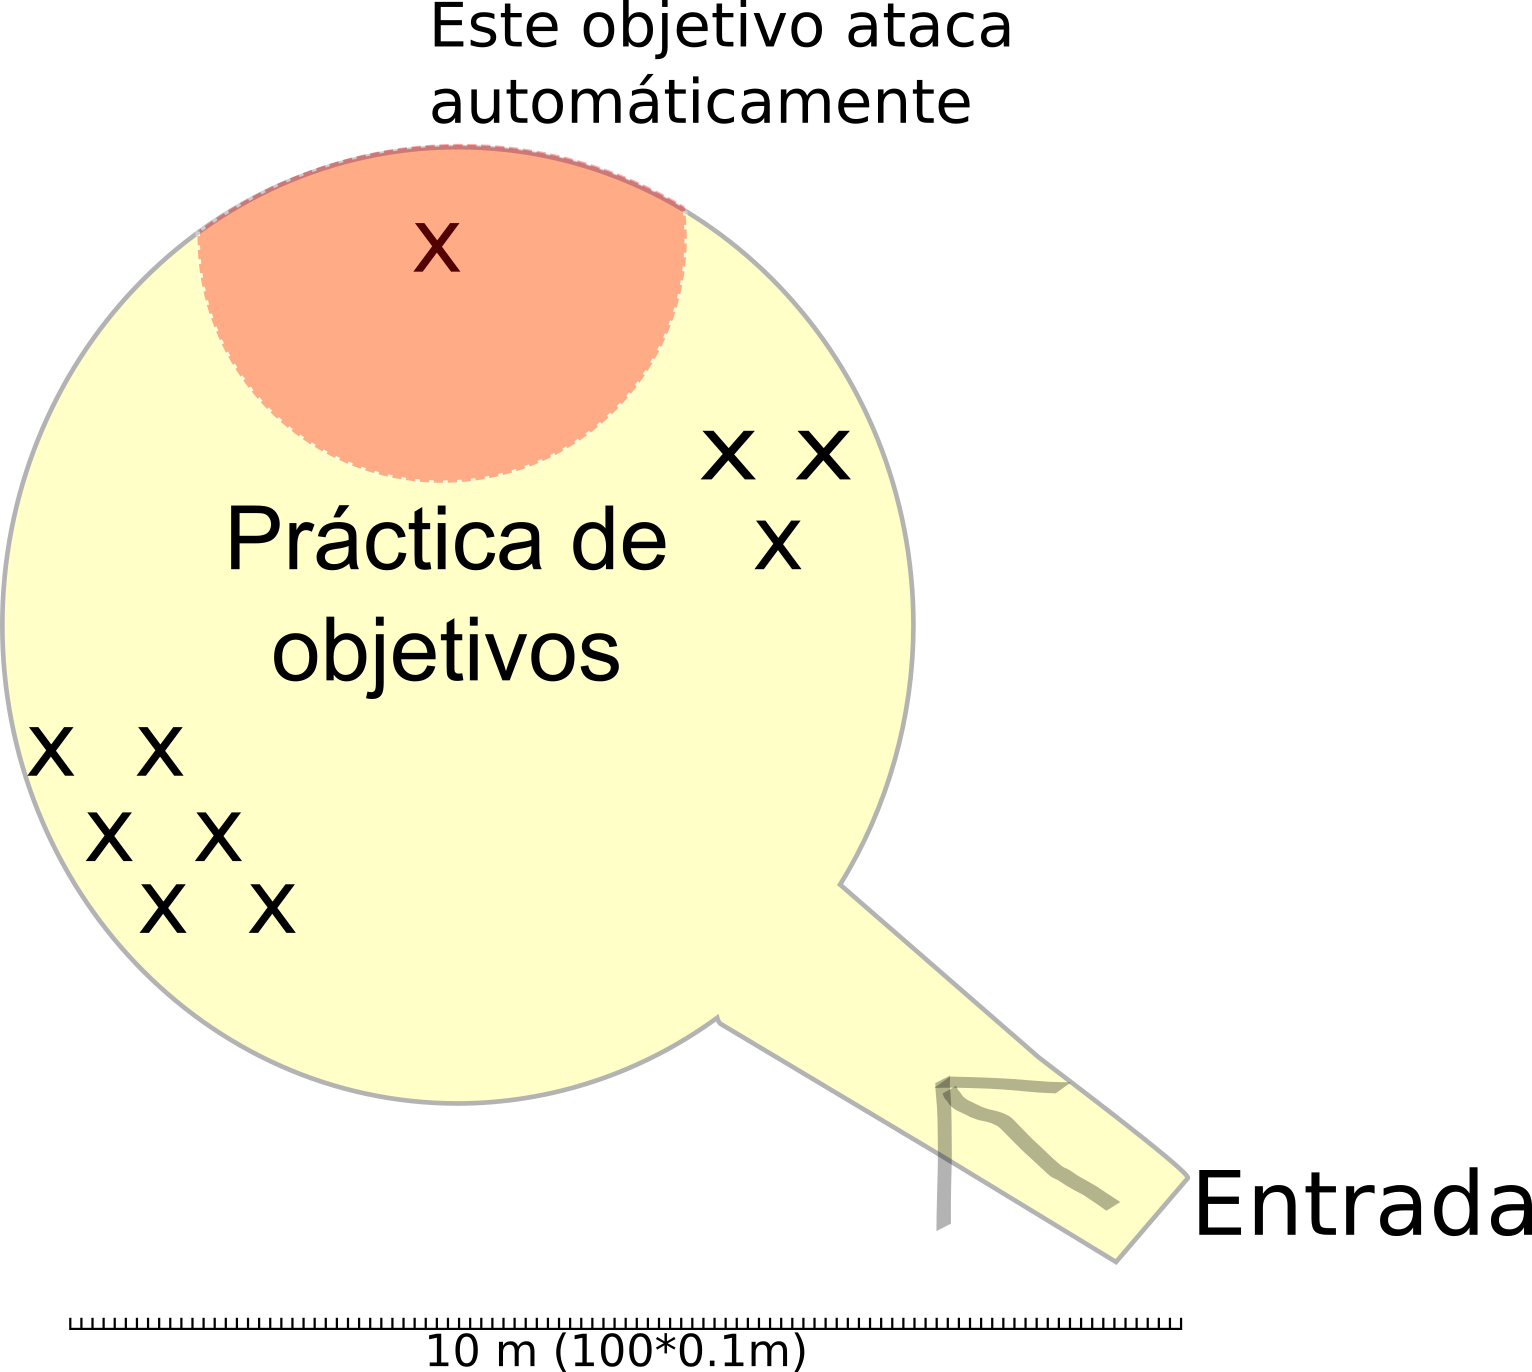
\includegraphics[width=0.8\textwidth]{tutorial}
    \caption{Un nivel de tutorial}
\end{figure}


\begin{figure}[H]
    \centering
    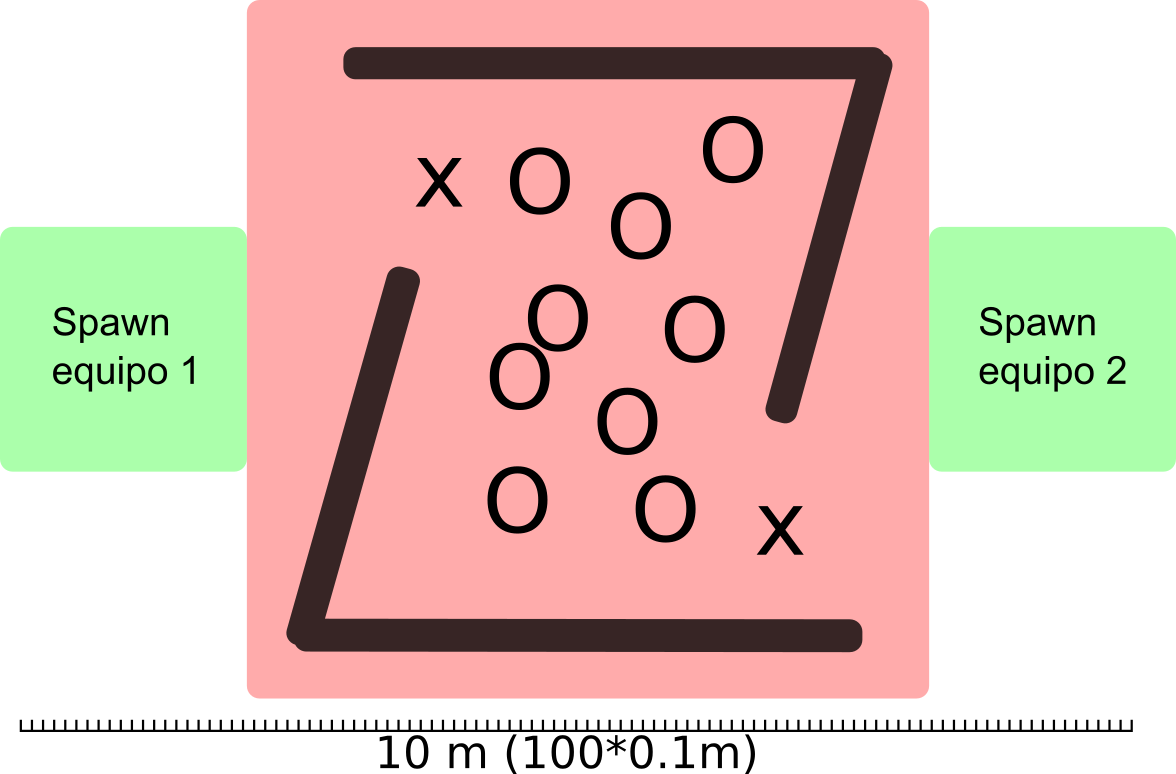
\includegraphics[width=0.7\textwidth]{flags}
    \caption{Un nivel de CTF. Las X representan banderas y los círculos son coberturas destructibles.}
\end{figure}

\subsection{Replay Appeal}

El juego debe ser constantemente rejugable. Para ello se incluyen quests diarias para reclamar la atención regular del jugador combinado con un gameplay ajustado y dinámico.

\subsection{Longevity}

La esperanza de vida del juego queda definida como 10.000 jugadores online diarios, ó 7 jugadores buscando partida por minuto, ó 1 partida formándose por minuto. Llegado este punto el juego online es claramente insostenible y la expectativa es que el juego tarde 4 años en decaer a éste nivel de juego.

\subsection{Save system}

Todos los datos de juego (desbloqueos y personalización) se guardan en un sistema de servidores remoto que será accedido por el juego para matchmaking.

\newpage

\section{Multiplayer}

\subsection{Native Multiplayer}

El juego permite a jugadores juntarse en una casa, conectar la Nintendo Switch y jugar en pantalla partida compartiendo un televisor. Los jugadores pueden loguearse en sus propias cuentas y usarlas en la consola de un amigo o bien usar una copia del personaje del dueño de la consola con colores cambiados.

\subsection{External Multiplayer}

Es el modo básico del juego, multijugador online.

\newpage

\section{Network}

\subsection{Network Functions}

Como ya se ha comentado, la base del juego es el multijugador online.

\subsection{Downloadable Content}               

Con el fin de extender la vida útil del juego se proveerá a los jugadores con contenido desbloqueable a posteriori del lanzamiento, como nuevos skins y habilidades.

\subsection{HOME}

Dado que no es un juego para PS3, no contiene funciones extra de HOME. Contenido para el equivalente de Nintendo Switch, la Mii Plaza, se considerará a posteriori del lanzamiento del juego.

\newpage
\section{State of the Art}
\subsection{La Competencia}
Este juego compite directamente con otros shooters multijugador competitivos como \textit{Call of Duty}, \textit{Battlefield}, \textit{S3 League} (éste en 3ª persona también), \textit{Counter Strike} etc. También entra en el mercado de los Multiplayer Online Battle Arena (MOBAs) y otros tipos de videojuego altamente competitivos, como \textit{DOTA} y \textit{LOL}. Dado que la temática es mágica-medieval también podría ocupar espacio de mercado de juegos de fantasía altamente centrados en gameplay en 3ª persona como \textit{Dark Souls}.

Nuestra mayor competencia directa es el shooter multijugador competitivo en 3ª persona de Nintendo, \textit{Splatoon}. 

\subsection{Superando la Competencia: Unique Selling Points}
Para convencer a la gente que está jugando los juegos arriba mencionados optaremos por aprovechar:

\begin{itemize}
\item La combinación de shooter altamente competitivo con una ambientación fantástica, que no ha sido probada aún en el mercado.
\item Gameplay sólido con control altamente responsivo
\item Situaciones espectaculares que hacen fácil que el juego se promocione a sí mismo en redes sociales, mediante el reenvío de gifs o vídeos con jugadas llamativas
\item Personalización en todos los aspectos del juego (desde habilidades hasta apariencia)
\end{itemize}

\newpage

\section{Milestone Schedule}

\cleardoublepage

\thispagestyle{empty}

\vspace*{\fill}

\begin{figure}[h]
    \centering
    
\includegraphics[width=0.6\textwidth]{fireball}
\end{figure}

\vfill

\end{document}
